\chapter{Introduction}

\section{Introduction to Reinforcement Learning}
\begin{flushleft}
People and animals learn by interacting with their environment. The difference between RL and other learning methods is that:
\begin{compactitemize}
\item The learning is active rather than passive.
\item Interactions are sequential rather than independent.
\item We are goal-oriented.
\item We can learn without examples of optimal behaviour.
\item Instead of examples, we mostly optimize a reward signal.
\end{compactitemize}
\end{flushleft}

\subsection{Characteristics of Reinforcement Learning}
\begin{flushleft}
    Reinforcement learning differs fundamentally from other machine learning paradigms through its unique structural characteristics. The absence of a supervisor represents perhaps the most significant distinction, as agents receive only scalar reward signals rather than explicit correct answers or labeled examples. This creates an environment where learning must occur through exploration and experimentation.
    
    The temporal dimension introduces complexity through delayed feedback mechanisms. Unlike supervised learning where feedback is immediate, reinforcement learning agents must navigate scenarios where the consequences of actions may not manifest for extended periods. This delay creates challenges in understanding cause-and-effect relationships and requires sophisticated approaches to credit assignment.
    
    The sequential and non-independent nature of data violates fundamental assumptions underlying many traditional machine learning approaches. Each decision influences the environment and subsequently affects the data the agent will encounter, creating a dynamic feedback loop that requires specialized algorithmic approaches.
\end{flushleft}

\subsection{Rewards and the Reward Hypothesis}
\begin{flushleft}
    The reward signal $R_t$ serves as the fundamental feedback mechanism in reinforcement learning, providing a scalar value that quantifies agent performance at each time step $t$. The primary objective for any reinforcement learning agent involves maximizing cumulative reward over time, transforming diverse goals into a unified optimization framework.
    
    The theoretical foundation rests on the Reward Hypothesis, which posits that all objectives and goals can be expressed through the maximization of expected cumulative reward. This hypothesis provides mathematical tractability and enables the application of optimization techniques across diverse domains.
    
    Practical applications demonstrate the versatility of reward-based formulations. Autonomous systems like helicopter control use positive rewards for trajectory following and negative rewards for safety violations. Game-playing applications assign rewards based on wins and losses, while financial systems reward profitable outcomes. These examples illustrate how complex objectives can be reduced to scalar signals that guide learning.
\end{flushleft}

\subsection{Sequential Decision Making and Long-term Planning}
\begin{flushleft}
    The core challenge in reinforcement learning involves selecting actions that maximize total future reward rather than immediate gratification. This temporal perspective requires agents to consider long-term consequences of current decisions, often necessitating short-term sacrifices for greater future benefits.
    
    The credit assignment problem represents a fundamental challenge in understanding which specific actions contributed to received rewards. When rewards are delayed, agents must develop mechanisms to attribute success or failure to appropriate historical decisions. This becomes particularly complex in scenarios with extended temporal horizons where multiple actions may collectively influence outcomes.
    
    Strategic thinking emerges naturally from this framework, as agents learn to make decisions that may not provide immediate benefits but enhance long-term prospects. Financial investments exemplify this principle, where initial costs must be weighed against potential future returns. Similarly, preventive actions like helicopter refueling represent immediate costs that prevent future catastrophic failures.
\end{flushleft}

\begin{figure}[H]
    \centering
    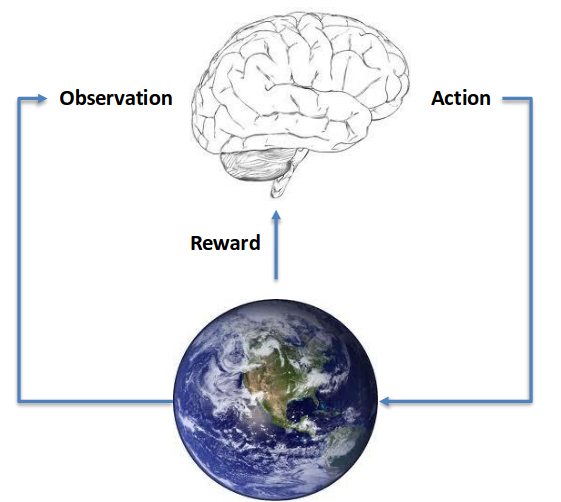
\includegraphics[width=0.5\textwidth]{images/AE.png}
    \caption{Interaction between agent and environment in reinforcement learning. At each time step $t$, the agent receives an observation $O_t$ and a scalar reward $R_t$, then executes an action $A_t$. The environment, in turn, receives the action $A_t$ and emits the next observation $O_{t+1}$ along with the reward $R_{t+1}$. The time index $t$ increments at each environment step, resulting in a continuous cycle of perception, action, and feedback that drives the agent's learning process.}
    \label{fig:rl_agent_environment}
\end{figure}

\section{History and State in Reinforcement Learning}

\subsection{The Role of History}
\begin{flushleft}
    The foundation of reinforcement learning dynamics lies in the concept of history, defined as the complete sequence of observations, actions, and rewards encountered by the agent up to any given time step. 
    \begin{equation}
    H_t = O_1, R_1, A_1, \ldots, A_{t-1}, O_t, R_t
    \end{equation}
    
    This history encompasses all observable variables that have occurred up to time $t$, creating a comprehensive record of the agent's interaction with its environment. The evolution of this history determines what happens next in the learning process, as both the agent's action selection and the environment's response depend fundamentally on this accumulated experience.
    
    The agent utilizes this historical information to select subsequent actions, while the environment processes the agent's actions to generate new observations and rewards. This creates a continuous cycle where past experiences inform future decisions, and future experiences expand the historical knowledge base available for decision-making.
\end{flushleft}

\subsection{State as a Function of History}
\begin{flushleft}
    While history provides complete information about past interactions, it quickly becomes unwieldy as the number of time steps increases. State emerges as a crucial abstraction that captures the essential information needed to determine future behavior. Formally, state is defined as a function of the history:
    $S_t = f(H_t)$.
    This functional relationship allows the agent to compress the potentially infinite sequence of past observations, actions, and rewards into a more manageable representation that retains the essential characteristics needed for decision-making. The choice of function $f$ becomes critical in determining how effectively the agent can learn and perform in its environment.
\end{flushleft}

\subsection{Environment State}
\begin{flushleft}
    The environment state $S_t^e$ represents the environment's private internal representation at time $t$. This encompasses whatever data the environment uses internally to determine the next observation and reward that will be provided to the agent. The environment state contains the complete information necessary for the environment to evolve according to its underlying dynamics.
    Typically, the environment state remains invisible to the agent, creating a fundamental information asymmetry in the learning process. Even when portions of the environment state become observable, they may contain substantial amounts of irrelevant information that do not directly influence the agent's decision-making process. This creates challenges in distinguishing between relevant and irrelevant environmental factors.
    The environment's internal representation often includes complex physical processes, hidden variables, and computational states that determine system behavior. In robotics applications, this might include precise motor positions, sensor calibrations, and physical dynamics that affect system response but remain hidden from the agent's direct observation.
\end{flushleft}

\subsection{Agent State}
\begin{flushleft}
    The agent state $S_t^a$ constitutes the agent's internal representation of the current situation, encompassing whatever information the agent uses to select its next action. This representation forms the foundation for all reinforcement learning algorithms, as it determines how the agent processes historical information and makes decisions.
    The agent state can be constructed as any function of the history:
    \begin{equation}
    S_t^a = f(H_t)
    \end{equation} This flexibility allows for diverse approaches to state representation, from simple memory-less strategies that only consider the current observation to sophisticated approaches that maintain complex internal models of environment dynamics.
    The quality of the agent state representation directly impacts learning performance and efficiency. Effective state representations capture relevant patterns in the environment while filtering out noise and irrelevant details. This balance between information retention and computational efficiency represents a key design consideration in reinforcement learning systems.
\end{flushleft}

\subsection{Information State and the Markov Property}
\begin{flushleft}
    An information state, also known as a Markov state, contains all useful information from the history necessary to predict future outcomes. A state $S_t$ satisfies the Markov property if and only if:
    \begin{equation}
         P[S_{t+1}|S_t] = P[S_{t+1}|S_1, \ldots, S_t]
    \end{equation}
    This mathematical condition captures the intuitive notion that "the future is independent of the past given the present." The Markov property creates a powerful simplification where the current state provides sufficient information to predict future behavior, allowing the entire history to be discarded once the state is known.
    The relationship can be visualized as: $H_{1:t} \rightarrow S_t \rightarrow H_{t+1:\infty}$, where the state $S_t$ acts as a sufficient statistic that captures all relevant information from the past history needed to predict future developments.     
    where the state $S_t$ acts as a sufficient statistic that captures all relevant information from the past history needed to predict future developments. This property proves essential for mathematical tractability in reinforcement learning algorithms.
    
    Both the environment state $S_t^e$ and the complete history $H_t$ naturally satisfy the Markov property. The environment state contains all information the environment uses for future evolution, while the history includes all possible relevant information by definition. However, constructing agent states that maintain the Markov property while remaining computationally tractable represents a central challenge in reinforcement learning.
\end{flushleft}

\section{Observability in Reinforcement Learning}

\subsection{Fully Observable Environments}
\begin{flushleft}
    Full observability occurs when the agent directly observes the complete environment state at each time step. In this scenario, the observation, agent state, and environment state become equivalent:
    \begin{equation}
    O_t = S_t^a = S_t^e
    \end{equation} This creates a transparent relationship between the agent's perception and the true state of the environment.
    Fully observable environments correspond formally to Markov Decision Processes (MDPs), which provide a mathematically tractable framework for reinforcement learning. The Markov property ensures that optimal decisions can be made based solely on current state information without requiring access to historical data.
    Examples of fully observable environments include many board games like chess or Go, where all relevant information remains visible to all players. Simple grid worlds and mathematical optimization problems also frequently satisfy full observability conditions, making them popular choices for developing and testing reinforcement learning algorithms.
\end{flushleft}

\subsection{Partially Observable Environments}
\begin{flushleft}
    Partial observability represents the more common and challenging scenario where agents indirectly observe the environment state through limited sensory information. In these situations, the agent state differs fundamentally from the environment state, creating information uncertainty that complicates decision-making.
    Real-world applications frequently involve partial observability. A robot navigating with camera vision lacks direct access to its precise global coordinates and must infer position from visual landmarks. Trading agents observe current market prices but cannot directly access the complete information driving market dynamics. Poker-playing agents see only public cards and their private hand while remaining unaware of opponents' cards and internal strategies.
    Partially observable environments correspond formally to Partially Observable Markov Decision Processes (POMDPs), which require more sophisticated solution techniques than standard MDPs. The agent must construct its own state representation $S_t^a$ that captures relevant information while managing uncertainty about hidden aspects of the environment.
    Several approaches exist for constructing agent states in partially observable environments. Complete history retention uses:
    \begin{equation}
    S_t^a = H_t
    \end{equation}
    maintaining all past information but potentially creating computational challenges as history length increases. Belief state approaches maintain probability distributions over possible environment states:
    \begin{equation}
    S_t^a = (P[S_t^e = s_1], \ldots, P[S_t^e = s_n])
    \end{equation}
    Modern approaches often employ recurrent neural networks to process sequential information:
    \begin{equation}
    S_t^a = \sigma(S_{t-1}^a W_s + O_t W_o)
    \end{equation}
    where $\sigma$ represents an activation function and $W_s, W_o$ are learned weight matrices.
    The choice of state representation strategy significantly impacts both learning efficiency and final performance in partially observable environments. Effective representations must balance information retention with computational tractability while adapting to the specific structure and dynamics of the target domain.
\end{flushleft}

\begin{figure}[H]
    \centering
    \begin{minipage}{0.45\textwidth}
        \centering
        
\includegraphics[width=\textwidth]{images/ex1.png}
        \label{fig:RL_Examples}
    \end{minipage}
    \hfill
    \begin{minipage}{0.4\textwidth}
        \centering
        
\includegraphics[width=\textwidth]{images/ex1_2.png}
        \label{fig:RL_Examples}
    \end{minipage}
    \label{fig:RL_Examples}
\end{figure}

\begin{flushleft}
    In the example above, the agent state is not a markov state, which means that the agent does not have access to all the information needed to make the best decision. The agent can only see what is around of it, and it cannot see what the whole map. This means that the agent cannot make the best decision because it does not have all the information it needs. In particulary the agent state in the two insighs position is the same,but the move to make is different.
\end{flushleft}

\section{Major Components of an RL Agent}

\begin{flushleft}
    A reinforcement learning agent may include one or more of the following fundamental components that define its architecture and capabilities. These components work together to enable the agent to perceive its environment, make decisions, and learn from experience. The specific combination and implementation of these components determine the agent's learning approach and performance characteristics.
\end{flushleft}

\subsection{Policy}
\begin{flushleft}
    A policy represents the agent's behavior function, serving as the core decision-making mechanism that maps from states to actions. The policy defines how the agent behaves at any given moment and constitutes the primary component that determines action selection in response to environmental observations.
    
    Given a state, the policy provides guidance on the best action or actions to take. This mapping can take different mathematical forms depending on the specific requirements and constraints of the learning problem.
    
    A deterministic policy provides a single action for each state:
    \begin{equation}
    a = \pi(s)
    \end{equation}
    where $\pi$ is the policy function that maps state $s$ directly to action $a$. This approach creates a clear, unambiguous decision rule but may lack the flexibility needed in uncertain environments.
    
    A stochastic policy defines a probability distribution over actions for each state:
    \begin{equation}
    \pi(a|s) = P[A_t = a | S_t = s]
    \end{equation}
    This formulation allows the agent to maintain uncertainty over action choices and enables exploration through probabilistic action selection. Stochastic policies prove particularly valuable in environments with incomplete information or when exploration is necessary for learning.
\end{flushleft}

\subsection{Value Function}
\begin{flushleft}
    The value function provides a prediction of future reward, serving as a mechanism to evaluate the goodness or badness of states and actions. This evaluation capability enables the agent to select actions based on their expected long-term consequences rather than immediate rewards.
    
    The state value function under policy $\pi$ is defined as:
    \begin{equation}
    v^\pi(s) = E[R_{t+1} + \gamma R_{t+2} + \gamma^2 R_{t+3} + \cdots | S_t = s]
    \end{equation}
    
    The discount factor $\gamma \in [0,1]$ controls the trade-off between immediate and long-term rewards. When $\gamma = 0$, the agent focuses entirely on immediate rewards, while $\gamma = 1$ weights all future rewards equally. Intermediate values create a preference for nearer rewards while still considering future consequences.
    
    Value functions serve multiple purposes in reinforcement learning. They enable the comparison of different states or actions based on their expected returns, provide a basis for policy improvement by identifying more valuable alternatives, and offer a mechanism for learning optimal behavior through value-based methods.
    
    Agents often approximate value functions when exact computation becomes intractable due to large state spaces or complex dynamics. Effective algorithms exist to learn these approximations efficiently, and with an accurate value function, agents can behave optimally. Even with suitable approximations, agents can achieve good performance in intractably large domains.
\end{flushleft}

\subsection{Model}
\begin{flushleft}
    A model predicts what the environment will do next, providing the agent with an internal representation of environmental dynamics. This predictive capability enables planning and forward-looking decision making, though it represents an optional component that not all reinforcement learning approaches require.
    
    The transition function $P$ predicts the next state given the current state and action:
    \begin{equation}
    P_{ss'}^a = P[S_{t+1} = s' | S_t = s, A_t = a]
    \end{equation}
    This probabilistic formulation captures the uncertainty inherent in many environments while providing expectations about state evolution.
    
    The reward function $R$ predicts the immediate reward expected from taking a specific action in a given state:
    \begin{equation}
    R_s^a = E[R_{t+1} | S_t = s, A_t = a]
    \end{equation}
    
    Together, these components create a complete model of environmental dynamics that can support various planning approaches. However, it's important to note that a model does not immediately provide a good policy. The agent must still engage in planning or other optimization processes to translate model predictions into effective action selection strategies.
    
    Model-based approaches offer several advantages including sample efficiency through simulated experience, the ability to reason about long-term consequences, and support for sophisticated planning algorithms. However, they also introduce challenges related to model accuracy, computational complexity, and the potential for model bias to negatively impact learning performance.
\end{flushleft}


\begin{figure}[H]
    \centering
    \begin{minipage}{0.3\textwidth}
        \centering
        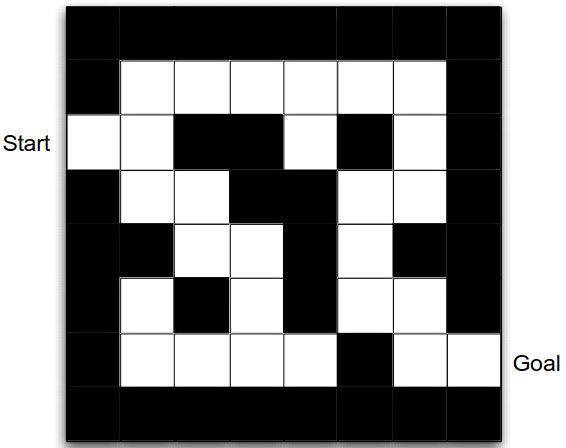
\includegraphics[width=\textwidth]{images/maze.png}
        \caption{Maze Examples}
        \label{fig:Maze_Examples}
    \end{minipage}
    \hfill
    \begin{minipage}{0.3\textwidth}
        \centering
        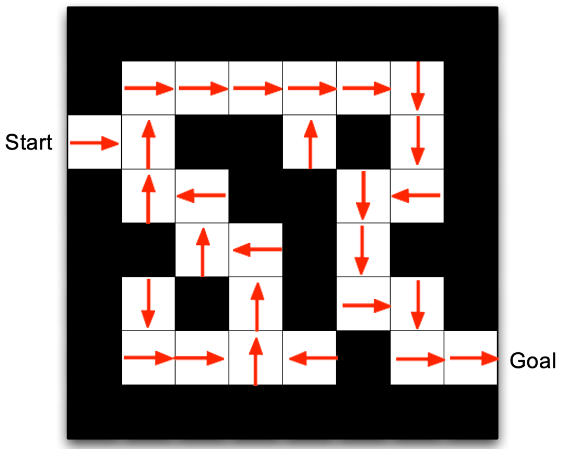
\includegraphics[width=\textwidth]{images/maze_policy.png}
        \caption{Maze Policy}
        \label{fig:Maze_Policy}
    \end{minipage}
    \label{fig:Maze_Examples}
\end{figure}


\begin{figure}[H]
    \centering
    \begin{minipage}{0.3\textwidth}
        \centering
        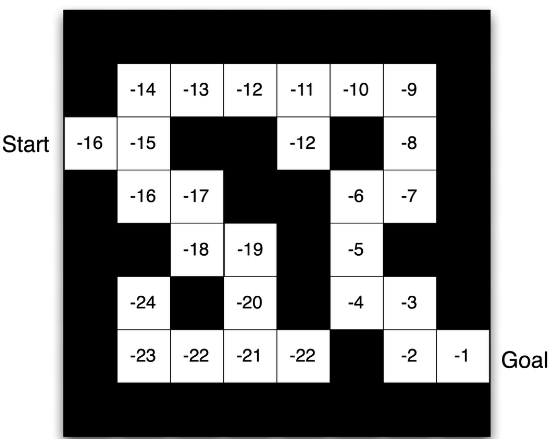
\includegraphics[width=\textwidth]{images/maze_value.png}
        \caption{Maze Value}
        \label{fig:Maze_Value}
    \end{minipage}
    \hfill
    \begin{minipage}{0.3\textwidth}
        \centering
        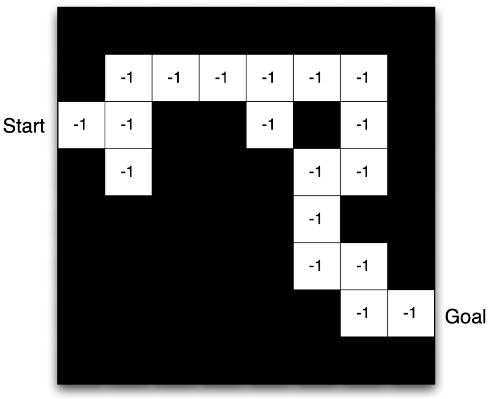
\includegraphics[width=\textwidth]{images/maze_model.png}
        \caption{Maze Model}
        \label{fig:Maze_Model}
    \end{minipage}
    \label{fig:Maze_model}
\end{figure}

\begin{flushleft}
    In the maze example above, reinforcement learning is illustrated through an agent that moves in the environment with four possible actions: north, east, south, and west, with its state corresponding to its position. Each step the agent takes incurs a penalty of -1, encouraging it to reach the goal in the fewest moves possible. The agent’s policy assigns an action to each state, represented by arrows in the cells, while the value function assigns a number to each state that reflects how advantageous it is to be there under the given policy. The agent may also build an internal model of the environment, describing how actions change the state and what rewards are received. This model, which represents the transition dynamics and the immediate rewards associated with states, can be imperfect or incomplete, but it helps guide decisions and predict the environment’s behavior.
\end{flushleft}

\section{Categorizing Reinforcement Learning Agents}

\begin{flushleft}
    Reinforcement learning agents can be systematically categorized based on their architectural components and learning approaches.
\end{flushleft}

\subsection{Component-Based Categorization}
\begin{flushleft}
    \textbf{Value-Based Agents} rely exclusively on value function estimation without maintaining an explicit policy representation. The policy emerges implicitly through greedy action selection from the value function.
    
    \textbf{Policy-Based Agents} maintain explicit policy representations without computing value functions, directly optimizing policy parameters to maximize expected returns.
    
    \textbf{Actor-Critic Agents} combine both policy and value function components. The critic estimates value functions while the actor maintains and updates the policy based on this feedback.
\end{flushleft}

\subsection{Model-Based vs Model-Free Categorization}
\begin{flushleft}
    \textbf{Model-Free Agents} learn directly from experience without constructing explicit models of environmental dynamics, reducing computational complexity but requiring more environmental interaction.
    
    \textbf{Model-Based Agents} construct internal models of environmental dynamics, enabling planning and achieving greater sample efficiency through simulated experience.
\end{flushleft}


\begin{figure}[H]
    \centering
    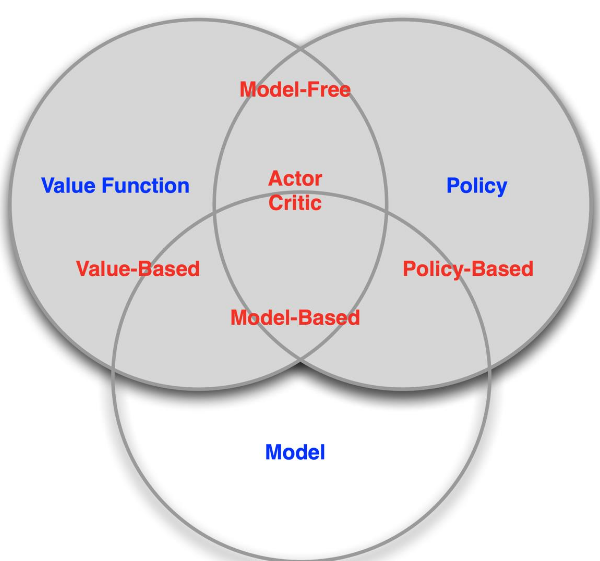
\includegraphics[width=0.4\textwidth]{images/RL_agent_taxonomy.png}
    \caption{Taxonomy of Reinforcement Learning Agents}
    \label{fig:RL_Agent_Taxonomy}
\end{figure}

\section{Learning and Planning in Reinforcement Learning}

\begin{flushleft}
    Sequential decision making encompasses two fundamental problem formulations that represent different approaches to optimizing agent behavior over time.
\end{flushleft}

\subsection{Reinforcement Learning}
\begin{flushleft}
    In reinforcement learning scenarios, the environment remains initially unknown to the agent. Learning occurs through direct interaction with the environment, where the agent observes states, executes actions, receives rewards, and uses this experience to improve its policy over time.
    
    This trial-and-error learning process requires the agent to balance exploration of unknown aspects of the environment with exploitation of current knowledge to maximize rewards. The agent must discover effective behaviors without access to optimal examples or complete environmental specifications.
    
    Real-world applications frequently exhibit these characteristics. Consider Atari game learning where the rules remain unknown initially. The agent must learn directly from interactive gameplay, selecting joystick actions and observing resulting pixels and scores. Through repeated interaction, the agent gradually discovers effective strategies without prior knowledge of game mechanics.
\end{flushleft}

\subsection{Planning}
\begin{flushleft}
    Planning scenarios assume complete knowledge of environmental dynamics through available models. The agent performs computational optimization using its model without requiring external environmental interaction during the planning phase. This enables the agent to simulate potential futures and optimize policies through internal computation.
    
    Planning approaches prove valuable when accurate models exist or can be constructed from limited data. In the Atari context, if complete game rules were known, the agent could query an internal emulator to determine the consequences of potential actions. This perfect model enables the agent to plan ahead using techniques such as tree search to identify optimal policies.
    
    The key distinction lies in information availability: reinforcement learning addresses unknown environments through interaction, while planning leverages known environmental models through computation.
\end{flushleft}

\section{Exploration and Exploitation}

\subsection{The Exploration-Exploitation Dilemma}
\begin{flushleft}
    Reinforcement learning resembles trial-and-error learning where agents must discover effective policies while minimizing reward loss during learning. The central challenge involves balancing exploration (gathering information about the environment) with exploitation (leveraging current knowledge to maximize rewards).
\end{flushleft}

\subsection{Examples}
\begin{flushleft}
    This trade-off appears across many domains: restaurant selection (favorite vs new restaurant), online advertising (successful vs experimental ads), and game playing (believed optimal vs exploratory moves).
\end{flushleft}

\section{Prediction and Control}

\begin{flushleft}
    Reinforcement learning problems naturally divide into two complementary categories that address different aspects of sequential decision making.
\end{flushleft}

\subsection{Prediction Problems}
\begin{flushleft}
    Prediction problems focus on evaluating future performance under given policies. The agent receives a specific policy and must determine its expected performance characteristics. This evaluation process requires estimating value functions that quantify long-term rewards achievable under the specified policy.
    
    Prediction serves multiple purposes including policy comparison, understanding environmental dynamics, and providing baselines for policy improvement algorithms. Accurate prediction capabilities enable agents to assess policy quality and identify areas for potential improvement.
\end{flushleft}


\begin{figure}[H]
    \centering
    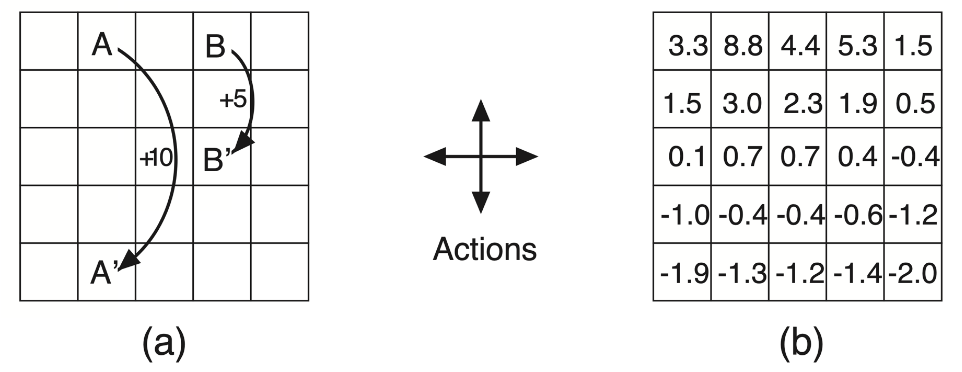
\includegraphics[width=0.5\textwidth]{images/prediction_ex.png}
    \caption{Prediction problem example}
    \label{fig:Prediction_Problem_Example}
\end{figure}


\subsection{Control Problems}
\begin{flushleft}
    Control problems address policy optimization without predetermined behavioral specifications. The agent must discover optimal policies through interaction and learning, combining prediction capabilities with policy improvement mechanisms.
    
    Control represents the ultimate goal of most reinforcement learning applications, where agents must autonomously discover effective behaviors. This requires sophisticated algorithms that can simultaneously evaluate current policies and identify improvements through exploration and value function updates.
\end{flushleft}


\begin{figure}[H]
    \centering
    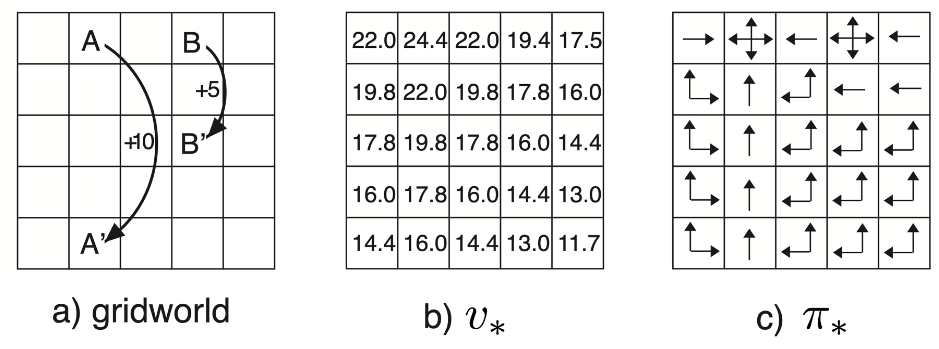
\includegraphics[width=0.5\textwidth]{images/controlo_ex.png}
    \caption{Control problem example}
    \label{fig:Control_Problem_Example}
\end{figure}


\section{Deep Reinforcement Learning}

\begin{flushleft}
    The integration of deep learning techniques with reinforcement learning creates powerful approaches for handling complex, high-dimensional problems that traditional methods cannot address effectively.
\end{flushleft}

\subsection{Function Approximation with Neural Networks}
\begin{flushleft}
    All major reinforcement learning components can be represented as functions suitable for neural network approximation.
    \begin{compactitemize}
        \item Policies map states to actions: $\pi: S \rightarrow A$. 
        \item Value functions map states to real-valued estimates: $v: S \rightarrow \mathbb{R}$. 
        \item Models map states to next states and rewards: $P: S \rightarrow S$ and $r: S \rightarrow \mathbb{R}$.    
    \end{compactitemize}
    Neural networks provide flexible function approximators capable of learning complex mappings from high-dimensional inputs. This enables reinforcement learning agents to handle image observations, continuous action spaces, and environments with millions of states.
\end{flushleft}

\subsection{Challenges in Deep Reinforcement Learning}
\begin{flushleft}
    Deep reinforcement learning violates fundamental assumptions underlying supervised learning approaches. The independent and identically distributed (i.i.d.) assumption fails because sequential decisions create correlated data where current actions influence future observations. Stationarity assumptions break down as the agent's changing policy modifies the data distribution over time.
    
    These violations require specialized techniques to ensure stable learning. Methods include experience replay to decorrelate training data, target networks to provide stable learning targets, and regularization approaches to handle non-stationary distributions. Successfully addressing these challenges enables deep reinforcement learning to achieve remarkable performance across diverse domains including game playing, robotics, and autonomous systems.
\end{flushleft}